\documentclass[12pt]{article}

% ---- Page geometry ----
\usepackage[margin=1in]{geometry}

% ---- Font and encoding ----
\usepackage[T1]{fontenc}
\usepackage{mathptmx}           % Times New Roman-style font (common in econ journals)

% ---- Spacing ----
\usepackage{setspace}
\doublespacing

% ---- Math ----
\usepackage{amsmath}

% ---- Tables ----
\usepackage{booktabs} % for \toprule, \midrule, \bottomrule
\usepackage{array}
\usepackage{float}              % for [H] placement
\usepackage{tabularray}         % required by modelsummary default output
\usepackage{siunitx}            % required by modelsummary default output
\SetTblrInner{rowsep=0pt} % tighten rows and shrink font in all tabularray tables

% ---- Graphics ----
\usepackage{graphicx}

% ---- Hyperlinks and references ----
\usepackage[hyphens]{url}
\usepackage[hidelinks]{hyperref}
\usepackage{microtype}

% ---- Bibliography style ----
\usepackage{natbib}
\bibliographystyle{aer}         % AER-style citations; can switch to chicago, etc.

% ---- Miscellaneous ----
\usepackage{enumitem}
\usepackage{caption}

% ---- Title block ----
\title{\textbf{What Drives Income Shifting by Multinational Enterprises?}}
\author{Brent Myers\thanks{University of Oklahoma. Email: \texttt{brent.t.myers-1@ou.edu}. This paper was prepared for Econ 5253: Data Science for Economists, Spring 2026.}}
\date{\today}

% =========================================================================
\begin{document}

\maketitle

% ---- Abstract ----
\begin{abstract}
\noindent This study examines the evolution of income shifting practices among U.S.\ multinational enterprises (MNEs) from 2010 to 2024, focusing on the influence of tax rate differentials between domestic and foreign jurisdictions, firm-specific characteristics, and the effects of the Tax Cuts and Jobs Act (TCJA) of 2017. Using Compustat data on 1,553 firm-year observations (346 unique firms), the analysis constructs a foreign-versus-domestic profitability differential as a proxy for income shifting. OLS estimation with robust standard errors reveals that tax differentials are the strongest predictor of income shifting, with higher foreign tax rates significantly reducing outbound shifting. Worldwide profitability is negatively associated with income shifting, while leverage and advertising intensity are positively associated. No statistically significant time trend or post-TCJA effect is detected. These findings are robust to year and industry fixed effects, TCJA interaction terms, and a sensitivity analysis excluding ambiguously classified geographic segments.

\medskip
\noindent \textbf{Keywords:} income shifting, transfer pricing, multinational enterprises, Tax Cuts and Jobs Act, tax differential
\end{abstract}

\newpage

% =========================================================================
\section{Introduction}

As globalization continues to increase, multinational enterprises (MNEs) are expanding operations across borders to capitalize on new economic growth opportunities. Meanwhile, firms historically focused on domestic markets are increasingly internationalizing to reach broader consumer bases and drive expansion. According to the \citet{imf2025} and other global economic outlooks, the global economy continues to steadily grow, albeit at slower rates currently due to significant geopolitical headwinds. The \citet{wef2025} notes that geo-economic fragmentation and geopolitical polarization continue to impact countries and communities, while exponential innovation across interconnected technologies offers unprecedented opportunities to increase productivity and standards of living. Barring unforeseeable global events, experts predict this trend of globalization and cross-border economic activity will continue steadily if not robustly.

Meanwhile, palpable tensions which have existed for decades among U.S.\ policymakers and MNEs continue to strengthen as policymakers accuse MNEs of not paying their fair share of taxes. Policymakers claim that MNEs are avoiding corporate taxes through ``legalized'' cross-border sheltering of profits. By sheltering of profits, they mean MNEs are shifting their income out of the U.S.\ into subsidiaries located in lower-taxed countries in order to avoid paying their fair share of taxes in the U.S. In a 2015 United States Senate budget report, \citet{sanders2015} argued that the largest corporations must pay their fair share rather than sheltering profits in offshore tax havens, particularly at a time of record-breaking corporate profits and rising inequality.

More recently, the \citet{taxjustice2024} reports that nearly half a trillion dollars is lost to tax havens each year by the largest firms in eight of the world's largest countries who refuse to curb global tax abuse. According to this report, the U.S.\ remains one of the worst offenders despite passing a sweeping overhaul of U.S.\ foreign tax legislation in 2017. The Tax Cuts and Jobs Act (TCJA) of 2017 fundamentally changed the taxation of U.S.\ multinational entities' foreign income \citep{chodorowreich2024} by introducing several major provisions aimed at making the U.S.\ tax system more competitive while also addressing long-standing incentives for shifting income and profits offshore.

This continued global expansion and ongoing tax policy tension intensifies the importance of understanding how MNEs manage their international tax burdens through transfer pricing policies. Transfer pricing is the pricing of transactions among affiliated entities and remains the key channel through which MNEs may shift income across jurisdictions to optimize tax outcomes. This study examines the evolution of income shifting practices among MNEs---focusing on the influence of tax rate differentials between domestic and foreign jurisdictions. It also investigates the role of firm-specific characteristics in shaping these behaviors and evaluates the effects of recent tax legislation on overall income shifting patterns.


% =========================================================================
\section{Literature Review}

Income shifting through transfer pricing remains a central strategy for MNEs seeking to optimize global taxation. While being somewhat mixed, the extensive prior literature provides evidence that MNEs engage in tax-motivated cross-jurisdictional income shifting by manipulating intracompany transaction prices and other transfers to allocate profits toward low-taxed jurisdictions without violating arms-length pricing rules \citep{harris1993, collins1998, klassen2012}.

\citet{harris1993}, \citet{collins1998}, and \citet{klassen2012} provide foundational evidence of MNEs exploiting the differential between U.S.\ and foreign statutory tax rates through income shifting in or out of the U.S. They find that firms with foreign tax rates exceeding the U.S.\ tax rate tend to shift income into the U.S., while firms facing lower foreign tax rates shift income out to foreign jurisdictions. \citet{harris1993} further investigated whether and how firm-specific characteristics like income-shifting flexibility or greater intangible assets affect income shifting. Additionally, he researched the impact of the U.S.\ Tax Reform Act (TRA) of 1986 on MNE income shifting. His findings suggest that tax law revisions can encourage strategic income shifting behavior with firm-specific attributes moderating the reaction. \citet{klassen2012} find clear evidence that U.S.\ MNEs have become more aggressive in shifting income out of the U.S.\ over time.

More recently, \citet{dyreng2023} explain that extant literature shows that MNEs engage in tax-motivated cross-jurisdictional income shifting, that cross-sectional variations identify conditions that enable or restrain income shifting, that intangible asset-heavy firms have more incentives to shift profits across borders, and that income shifting has generally increased over time as globalization has developed.

Together, these studies frame a theoretical foundation emphasizing that income shifting is influenced by tax rate differentials, firm-specific factors such as asset intangibility and operational flexibility, and regulatory environments. This foundation motivates the present research to analyze how income shifting has changed over time, how differences between domestic and foreign tax rates influence these strategies, the impact of firm-specific characteristics on income shifting, and the effects of recent tax legislation on overall shifting patterns.

Guided by prior literature, the following hypotheses are postulated.

\paragraph{Hypothesis 1 (Change Over Time and Regulatory Impact):}
Income shifting behavior among MNEs has changed over time with an overall increasing trend prior to TCJA, followed by a moderation or decline post-TCJA. This moderation is expected due to the tax legislation lowering the U.S.\ statutory rate and the introduction of other measures (e.g., GILTI rules, BEAT calculations, and FDII deductions) meant to curb income shifting and incentivize keeping intangible property in the U.S.

\paragraph{Hypothesis 2 (Tax Differential Effect):}
MNEs are more likely to shift income from jurisdictions with higher tax rates to those with lower tax rates. Therefore, as the tax differential increases the measured income shifting will likewise increase, although the strength and direction of this relationship may vary in the post-TCJA tax environment.

\paragraph{Hypothesis 3 (Firm Characteristics and Income Shifting):}
Firms with greater income-shifting flexibility, particularly those with higher intangible asset intensity, demonstrate stronger income shifting behaviors than firms with more tangible or inflexible asset bases.


% =========================================================================
\section{Data}

\subsection{Sample}

Drawing upon Compustat North America Fundamentals Annual data and WRDS Compustat Segment Merged file (part of the Compustat North America / Global Segment data), the final sample comprises MNEs with sufficient disclosure on financial statement and transfer pricing transactions (foreign segment data).

It consists of 1,553 firm-year observations (346 unique firms) from 2010--2024, a period spanning the 2017 enactment of the Tax Cuts and Jobs Act (TCJA). To ensure more statistically robust analysis, the data have been winsorized and missing variables have been addressed. The dependent variable, \textit{income\_shift}, is a foreign profitability differential measure as mentioned previously. With a mean of $0.0065$, it indicates minimal income shifting overall out of the U.S. Key independent variables include tax differential, worldwide profitability, firm size, leverage, R\&D intensity, advertising intensity, PPE intensity, a linear time trend (\textit{year\_trend}), and a post-TCJA indicator.

\subsection{Variable Construction}

Consistent with \citet{collins1998}, the measure for income shifting (\textit{income\_shift}) is foreign pre-tax income divided by foreign sales (foreign profitability) minus domestic pre-tax income divided by domestic sales (domestic profitability). Using this profitability differential as a proxy for income shifting is motivated by the fact that intracompany transfer prices that shift income into (out of) foreign subsidiaries result in relatively higher (lower) reported foreign profitability. This ratio directly reflects transfer pricing incentives because abnormal foreign profitability signals income being shifted across borders.

Also following \citet{collins1998}, worldwide profitability (\textit{ww\_profit}) and tax differential (\textit{tax\_diff}) are constructed. Worldwide profitability is used as a control variable for cross-sectional variation in a firm's overall profitability. It is calculated as worldwide pre-tax income divided by worldwide sales. Tax differential plays a central role as a key tax incentive variable explaining income shifting variation. It is calculated as the firm-specific weighted average foreign effective tax rate minus the U.S.\ statutory tax rate. It is of significant interest because it measures the incentive to shift income between the U.S.\ and foreign jurisdictions. This variable will allow the second hypothesis to be analyzed.

In an effort to capture the effect of time and the regulatory impact of TCJA, a linear time trend (\textit{year\_trend}) and a post-TCJA indicator (\textit{post\_tcja}) are added to the model. These variables will permit the analysis of the first hypothesis.

Firm-specific characteristics of size, leverage, research and development intensity, advertising intensity, and property, plant, and equipment intensity are also added to test the third hypothesis.

\textit{Firm size} is measured as the natural log of total assets. Because firm size may affect the desire to shift income, it is included as an explanatory variable. Its impact is ambiguous: larger firms may be inclined to shift more or possibly less income. Bigger firms have more resources to hire sophisticated tax advisors to construct complex international tax planning structures, and they have more global operations and therefore more opportunities to shift income. However, larger firms may face greater scrutiny from tax authorities and news media, and they are likely to have better governance and compliance culture leading them to engage in less income shifting.

\textit{Leverage} is measured as the firm's total debt divided by total assets. Leverage is included as a control variable because it may also affect income shifting. Leverage and income shifting could be seen as either substitutes or complements. Firms can reduce taxes through either income shifting or debt shifting (placing debt in high-tax jurisdictions and deducting interest), in which case leverage is a substitute. Alternatively, firms aggressive in one tax strategy (debt) may also be aggressive in others (income shifting), in which case leverage is a complement.

\textit{R\&D intensity} is the total R\&D expenses divided by total sales. R\&D generates intellectual property (patents, technology, know-how). These intangible assets are hard to value objectively, easier to relocate legally, and highly profitable---and therefore are a primary channel used to shift income.

\textit{Advertising intensity} is the total advertising expenditure divided by total sales. As advertising creates intangible assets (brand value, customer relationships, market reputation) similar to how R\&D creates intellectual property, it is included in the model. It is an alternative measure of asset intangibility and captures an element that might facilitate income shifting.

\textit{PPE intensity} is the total PPE (property, plant, and equipment) expense divided by total assets. Physical assets (factories, equipment, buildings) are considered immobile---tied to specific locations. PPE reduces income shifting opportunities. Therefore, capital-intensive firms (high PPE) are expected to engage in less income shifting.

\subsection{Descriptive Statistics}

Figure~\ref{fig:shift_time} illustrates the evolution of mean income shifting over the sample period, showing an upward trend pre-TCJA with greater volatility in the post-TCJA years. Figure~\ref{fig:tax_scatter} depicts the negative relationship between the tax differential and income shifting, with fitted regression lines for both the pre- and post-TCJA periods.

Table~\ref{tab:summary} in the Appendix shows the summary statistics for all the variables used in the regression analysis. A few noteworthy items are mentioned next.

The mean of the income shifting measure is slightly positive ($0.0065$) with a median near zero ($0.0097$), suggesting that on average, firms in the sample report marginally higher foreign profit margins relative to domestic profit margins. The measure exhibits a moderate standard deviation (0.1802). This suggests that income shifting behavior varies across the firms and years in the sample.

The tax differential variable has a mean of 0.0355, indicating that foreign effective tax rates in the sample average approximately 3.6 percentage points higher than the U.S.\ statutory rate across this sample period. However, the median is negative ($-0.0222$), revealing that the typical firm faces foreign tax rates slightly below the U.S.\ rate. This divergence between mean and median may reflect the structural change following the Tax Cuts and Jobs Act passed in 2017 as it reduced the U.S.\ corporate tax rate from 35\% to 21\%. Prior to the reform, most firms likely faced lower foreign tax rates (median negative), creating incentives for outbound income shifting. Post-reform, the reduced U.S.\ rate may have reversed these incentives for many firms, though some continue to operate in high-tax foreign jurisdictions. The variable's large standard deviation (0.2512) demonstrates that firms face markedly different tax rate differentials across jurisdictions and time periods, providing varying incentives for income shifting strategies.

Worldwide profitability averages 11.75\% (median 9.70\%), reflecting healthy profit margins for U.S.\ multinationals in the sample. The substantial variation in profitability levels (standard deviation 9.29\%) provides important context for interpreting income shifting behavior, as more profitable firms may face different tax planning incentives and constraints than less profitable peers.

Overall, the sample appears to encompass a broad range of firm sizes, capital structures, profitability levels, and business models across multiple industries and time periods, ensuring that the results reflect diverse economic environments and tax planning opportunities.


% =========================================================================
\section{Empirical Methods}

Following the methodological approaches primarily developed by \citet{collins1998} and further refined by \citet{klassen2012}, this study constructs measures of income shifting and tax differentials. Building upon these foundations, firm-specific characteristics and a post-TCJA indicator are incorporated into the regression framework to empirically test the hypotheses. This allows for an analysis of income shifting behavior both longitudinally and cross-sectionally, leveraging the strengths of prior methodologies while adding some new variables of contemporary interest.

The baseline specification is:
\begin{align}
\textit{income\_shift}_{it} &= \beta_0 + \beta_1 \cdot \textit{tax\_diff}_{it} + \beta_2 \cdot \textit{ww\_profit}_{it} + \beta_3 \cdot \textit{size}_{it} \notag \\
&\quad + \beta_4 \cdot \textit{leverage}_{it} + \beta_5 \cdot \textit{rnd\_intensity}_{it} + \beta_6 \cdot \textit{ad\_intensity}_{it} \notag \\
&\quad + \beta_7 \cdot \textit{ppe\_intensity}_{it} + \beta_8 \cdot \textit{year\_trend}_{t} + \beta_9 \cdot \textit{post\_tcja}_{t} + \varepsilon_{it}
\label{eq:model}
\end{align}
where subscripts $it$ denote firm $i$ in year $t$. Each variable is of interest as they each help to test the hypotheses and better understand the factors that affect MNE income shifting behaviors.


% =========================================================================
\section{Research Findings}

\subsection{Regression Model Estimation}

Table~\ref{tab:regression} in the Appendix presents the results of three model specifications: the baseline OLS model (Model~1), a year fixed effects specification (Model~2), and an interaction model testing whether the TCJA moderated key relationships (Model~3). Table~\ref{tab:industry_fe} reports Model~4, which adds industry fixed effects. Table~\ref{tab:sensitivity} presents a sensitivity analysis comparing the main sample to a restricted sample that excludes ambiguously classified geographic segments. The key findings and interpretations are discussed below.

\subsection{Interpretation of Results}

The overall regression model is jointly statistically significant ($F = 23.41$, $p < 0.0001$), indicating that the independent variables collectively explain variation in income shifting behavior. While the adjusted $R^2$ of 11.61\% may appear low, this is typical in transfer pricing and international tax research where firm behavior is influenced by many unobserved factors. The key findings are as follows.

\textit{Tax Differential} ($\hat{\beta} = -0.162$, $p < 0.0001$): This coefficient is negative and extremely significant, indicating that higher foreign tax rates relative to U.S.\ tax rates are associated with reduced income shifting incentives. This is consistent with theory and Hypothesis~2. Tax incentives are the strongest predictor of income shifting, confirming that firms respond rationally to tax rate differences across jurisdictions.

\textit{Worldwide Profitability} ($\hat{\beta} = -0.469$, $p < 0.0001$): This coefficient is also negative and significant, indicating that more profitable MNEs engage in less income shifting. This counterintuitive finding may be explained by highly profitable firms facing greater regulatory and public scrutiny or possessing legitimate competitive advantages that reduce their reliance on tax-motivated transfer pricing policies.

\textit{Advertising Intensity} ($\hat{\beta} = 0.231$, $p = 0.0118$): Advertising-intensive firms engage in more income shifting according to this positive and significant coefficient. Brand-based intangible assets, like R\&D-based assets, may facilitate transfer pricing flexibility through royalty payments, licensing fees, or cost-sharing arrangements, which would explain this significant finding. This supports Hypothesis~3.

\textit{Leverage} ($\hat{\beta} = 0.086$, $p < 0.0001$): Leveraged firms engage in more income shifting as shown by this significantly positive coefficient. This may suggest that firms use multiple tax strategies simultaneously---both debt financing (for interest deductions) and transfer pricing (for income shifting). Higher leverage may also indicate financial constraints that incentivize tax minimization.

\textit{Firm Size} ($\hat{\beta} = 0.005$, $p = 0.0488$): Larger firms engage in marginally more income shifting according to this positive and weakly significant coefficient. This is consistent with the view that larger firms have more global operations and greater resources to construct sophisticated international tax planning structures, providing more opportunities to shift income across jurisdictions.

R\&D intensity, PPE intensity, and year trend all show as insignificant. Although it is interesting to note that R\&D intensity has a negative coefficient, which is contrary to what was expected for this firm characteristic. Likewise, post-TCJA has a positive coefficient, which does not support Hypothesis~1. Additionally, year trend is insignificant, though its positive coefficient is directionally consistent with prior research findings.

\subsection{Year Fixed Effects and TCJA Interactions}

Model 2 adds year fixed effects to the baseline specification, replacing the linear time trend 
with individual year indicators. As shown in Table 2, the key coefficient estimates remain 
virtually unchanged from Model 1. The tax differential coefficient is still $-0.162$ ($p < 0.0001$) 
and worldwide profitability remains $-0.469$ ($p < 0.0001$). The stability of these estimates 
across specifications provides reassurance that the baseline results are not driven by 
unobserved year-specific shocks such as recessions, commodity price swings, or changes in 
global tax enforcement. The adjusted $R^2$ decreases slightly from 11.61\% to 11.22\%, suggesting that year-specific variation does not explain much additional variation in income shifting beyond what the linear trend already captures.

Model 3 introduces interaction terms between the post-TCJA indicator and three key 
variables: tax differential, R\&D intensity, and worldwide profitability. The purpose of 
these interactions is to test whether the TCJA fundamentally altered the relationship between 
these variables and income shifting. None of the three interaction terms are statistically 
significant. The tax differential interaction ($\hat{\beta} = -0.024$, $p > 0.10$) suggests 
that the sensitivity of income shifting to tax rate differences did not meaningfully change 
after the reform. Similarly, the R\&D intensity interaction ($\hat{\beta} = 0.069$, $p > 0.10$) 
and worldwide profitability interaction ($\hat{\beta} = 0.052$, $p > 0.10$) show no evidence 
that these relationships were moderated by the TCJA. Taken together, these results do not 
support Hypothesis 1 and suggest that while the TCJA reduced the U.S. statutory rate, it did 
not fundamentally change the underlying mechanisms through which firms shift income across 
jurisdictions.

\subsection{Industry Fixed Effects}

Model 4 adds two-digit SIC industry fixed effects to account for unobserved industry-level 
factors that may influence income shifting. As reported in Table 3, the inclusion of industry 
controls substantially increases the adjusted $R^2$ from 11.61\% to 33.62\%, indicating that 
industry membership explains a meaningful share of the variation in income shifting behavior. 
This is consistent with the expectation that certain industries, such as pharmaceuticals and 
technology, have more opportunities and incentives to shift income due to their reliance on 
intangible assets.

With industry effects included, the tax differential coefficient increases in magnitude to 
$-0.183$ ($p < 0.0001$), and the worldwide profitability coefficient nearly doubles to $-0.748$ 
($p < 0.0001$). Firm size also becomes more significant ($\hat{\beta} = 0.008$, $p < 0.01$). 
These changes suggest that after controlling for industry composition, the within-industry 
effects of tax incentives and profitability on income shifting are even stronger than the 
pooled estimates indicate. The remaining control variables retain their signs and general 
significance levels from Model 1, providing further evidence that the baseline results are 
robust to industry-level confounding.

\subsection{Sensitivity Analysis}

Table 4 presents a sensitivity analysis comparing the main sample to a restricted sample 
that excludes firm-year observations with ambiguously classified geographic segments. Some 
firms in Compustat report geographic segments using labels such as ``International,'' 
``Other,'' or regional groupings that do not clearly distinguish between domestic and foreign 
operations. These ambiguous classifications could introduce measurement error into the income 
shifting variable. The restricted sample contains 982 observations after removing these cases.

The core results are qualitatively unchanged in the restricted sample. The tax differential 
coefficient remains negative and highly significant ($\hat{\beta} = -0.152$, $p < 0.0001$), 
and worldwide profitability retains its negative and significant relationship with income 
shifting ($\hat{\beta} = -0.456$, $p < 0.0001$). Leverage also remains significant, though 
its magnitude decreases somewhat ($\hat{\beta} = 0.058$, $p < 0.01$). However, two variables 
that are significant in the main sample lose significance in the restricted sample: firm size 
($\hat{\beta} = 0.006$, $p > 0.10$) and advertising intensity ($\hat{\beta} = 0.090$, 
$p > 0.10$). This suggests that the significance of these variables in the full sample may be 
partly driven by observations where the geographic segment classification introduces noise into 
the dependent variable. Overall, the sensitivity analysis confirms that the primary conclusions 
regarding tax differentials and worldwide profitability are robust to alternative sample 
definitions, while the results for firm size and advertising intensity should be interpreted 
with some caution.

% =========================================================================
\section{Conclusion}

As the global business landscape continues to expand, the tension between policymakers and MNEs will remain strong until rigorous research sheds enough light on the evolution of income shifting practices. Understanding the influence of tax rate differentials between countries, the characteristics of firms that shape incentives, and the effect of tax legislation on income shifting patterns is the key to constructing productive incentives for firms to balance the paramount tradeoff between maximizing shareholder value through minimization of taxes paid and the responsibility to contribute appropriate tax amounts to fund the government. It is hoped that the results of this study are one small step in that direction.

In summary, the results show no significant time trend in income shifting, less income shifting at higher tax differentials (likely due to post-TCJA rules) and among highly profitable firms, greater shifting among larger firms and firms with higher leverage and advertising intensity, and no evidence that R\&D intensity or PPE intensity are related to income shifting in this sample.


% =========================================================================
\bibliography{references}

\medskip
\noindent\textit{AI Usage Note:} Generative AI tools (Perplexity, Claude) assisted with SAS coding for data gathering, cleaning, analysis, and limited text editing.


% =========================================================================
\appendix
\section*{Appendix}

% --- Table 1: Summary Statistics (auto-generated) ---
\begin{table}[H]
\centering
\caption{Summary Statistics for All Regression Variables}
\label{tab:summary}
\begin{tblr}[         %% tabularray outer open
note{}={Source: Compustat via WRDS. Sample period: 2010--2024, excluding 2017.},
]                     %% tabularray outer close
{                     %% tabularray inner open
colspec={Q[]Q[]Q[]Q[]Q[]Q[]Q[]},
hline{2}={1-7}{solid, black, 0.05em},
hline{1}={1-7}{solid, black, 0.08em},
hline{12}={1-7}{solid, black, 0.08em},
column{1}={}{halign=l},
column{2-7}={}{halign=r},
}                     %% tabularray inner close
& N & Mean & Median & SD & Min & Max \\
income\_shift & 1553 & \num{0.0065} & \num{0.0097} & \num{0.1802} & \num{-1.0000} & \num{1.0000} \\
tax\_diff & 1536 & \num{0.0355} & \num{-0.0222} & \num{0.2512} & \num{-0.3474} & \num{1.0000} \\
ww\_profit & 1553 & \num{0.1175} & \num{0.0970} & \num{0.0929} & \num{6.851e-04} & \num{1.0000} \\
size & 1553 & \num{7.8999} & \num{7.9067} & \num{1.9758} & \num{2.8613} & \num{14.6979} \\
leverage & 1553 & \num{0.2645} & \num{0.2212} & \num{0.2492} & \num{0.0000} & \num{2.4387} \\
rnd\_intensity & 1553 & \num{0.0209} & \num{0.0000} & \num{0.0437} & \num{0.0000} & \num{0.7584} \\
ad\_intensity & 1553 & \num{0.0137} & \num{0.0000} & \num{0.0356} & \num{0.0000} & \num{0.2821} \\
ppe\_intensity & 1553 & \num{0.2097} & \num{0.1453} & \num{0.1978} & \num{0.0013} & \num{0.8920} \\
year\_trend & 1553 & \num{5.7527} & \num{5.0000} & \num{4.3653} & \num{0.0000} & \num{14.0000} \\
post\_tcja & 1553 & \num{0.3670} & \num{0.0000} & \num{0.4822} & \num{0.0000} & \num{1.0000} \\
\end{tblr}
\end{table}


% --- Table 2: Models 1-3 Regression Results (auto-generated) ---
\newpage
\begin{spacing}{1.4}
\begin{table}[H]
\centering
\caption{OLS Regression Results --- Income Shifting Models (Robust Standard Errors)}
\label{tab:regression}
\begin{tblr}[         %% tabularray outer open
note{}={* p \num{< 0.1}, ** p \num{< 0.05}, *** p \num{< 0.01}},
note{ }={Heteroskedasticity-consistent (HC0) standard errors in parentheses.},
note{  }={Model 2 includes year fixed effects (2010 omitted); year\_trend and post\_tcja dropped due to collinearity.},
]                     %% tabularray outer close
{                     %% tabularray inner open
colspec={Q[]Q[]Q[]Q[]},
hline{2}={1-4}{solid, black, 0.05em},
hline{28}={1-4}{solid, black, 0.05em},
hline{1}={1-4}{solid, black, 0.08em},
hline{31}={1-4}{solid, black, 0.08em},
column{2-4}={}{halign=c},
column{1}={}{halign=l},
}                     %% tabularray inner close
& Model 1 & Model 2 & Model 3 \\
Intercept & \num{-0.026} & \num{-0.015} & \num{-0.022} \\
& (\num{0.021}) & (\num{0.024}) & (\num{0.022}) \\
tax\_diff & \num{-0.162}*** & \num{-0.162}*** & \num{-0.154}*** \\
& (\num{0.013}) & (\num{0.013}) & (\num{0.015}) \\
ww\_profit & \num{-0.469}*** & \num{-0.469}*** & \num{-0.491}*** \\
& (\num{0.091}) & (\num{0.091}) & (\num{0.112}) \\
size & \num{0.005}** & \num{0.005}* & \num{0.005}** \\
& (\num{0.003}) & (\num{0.003}) & (\num{0.003}) \\
leverage & \num{0.086}*** & \num{0.087}*** & \num{0.085}*** \\
& (\num{0.018}) & (\num{0.018}) & (\num{0.018}) \\
rnd\_intensity & \num{-0.092} & \num{-0.095} & \num{-0.108} \\
& (\num{0.101}) & (\num{0.101}) & (\num{0.123}) \\
ad\_intensity & \num{0.231}** & \num{0.232}** & \num{0.230}** \\
& (\num{0.092}) & (\num{0.092}) & (\num{0.092}) \\
ppe\_intensity & \num{0.047} & \num{0.046} & \num{0.046} \\
& (\num{0.035}) & (\num{0.034}) & (\num{0.035}) \\
year\_trend & \num{0.002} &  & \num{0.002} \\
& (\num{0.002}) &  & (\num{0.002}) \\
post\_tcja & \num{0.017} &  & \num{0.012} \\
& (\num{0.018}) &  & (\num{0.025}) \\
tax\_diff x post\_tcja &  &  & \num{-0.024} \\
&  &  & (\num{0.030}) \\
rnd\_intensity x post\_tcja &  &  & \num{0.069} \\
&  &  & (\num{0.216}) \\
ww\_profit x post\_tcja &  &  & \num{0.052} \\
&  &  & (\num{0.187}) \\
N & \num{1536} & \num{1536} & \num{1536} \\
R-squared & \num{0.1213} & \num{0.1237} & \num{0.1218} \\
Adj. R-squared & \num{0.1161} & \num{0.1122} & \num{0.1149} \\
\end{tblr}
\end{table}

\end{spacing}

% --- Table 3: Model 4 Industry FE (auto-generated) ---
\begin{table}[H]
\centering
\caption{OLS Regression with Industry Fixed Effects (Robust Standard Errors)}
\label{tab:industry_fe}
\begin{tblr}[         %% tabularray outer open
note{}={* p \num{< 0.1}, ** p \num{< 0.05}, *** p \num{< 0.01}},
note{ }={Heteroskedasticity-consistent (HC0) standard errors in parentheses.},
note{  }={Industry dummies based on 2-digit SIC codes (industries with <10 obs collapsed into Other).},
note{   }={Industry coefficients suppressed for brevity; jointly significant (p < 0.001).},
]                     %% tabularray outer close
{                     %% tabularray inner open
colspec={Q[]Q[]},
hline{2}={1-2}{solid, black, 0.05em},
hline{22}={1-2}{solid, black, 0.05em},
hline{1}={1-2}{solid, black, 0.08em},
hline{25}={1-2}{solid, black, 0.08em},
column{2}={}{halign=c},
column{1}={}{halign=l},
}                     %% tabularray inner close
& Model 4 \\
Intercept & \num{0.310}*** \\
& (\num{0.062}) \\
tax\_diff & \num{-0.183}*** \\
& (\num{0.014}) \\
ww\_profit & \num{-0.748}*** \\
& (\num{0.076}) \\
size & \num{0.008}*** \\
& (\num{0.003}) \\
leverage & \num{0.069}*** \\
& (\num{0.015}) \\
rnd\_intensity & \num{-0.147} \\
& (\num{0.118}) \\
ad\_intensity & \num{0.213}** \\
& (\num{0.105}) \\
ppe\_intensity & \num{0.035} \\
& (\num{0.027}) \\
year\_trend & \num{0.003} \\
& (\num{0.002}) \\
post\_tcja & \num{0.020} \\
& (\num{0.016}) \\
N & \num{1536} \\
R-squared & \num{0.3543} \\
Adj. R-squared & \num{0.3362} \\
\end{tblr}
\end{table}


% --- Table 4: Sensitivity Analysis (auto-generated) ---
\begin{table}[H]
\centering
\caption{Sensitivity Analysis --- Excluding Ambiguous Domestic Segments}
\label{tab:sensitivity}
\begin{tblr}[         %% tabularray outer open
note{}={* p \num{< 0.1}, ** p \num{< 0.05}, *** p \num{< 0.01}},
note{ }={Heteroskedasticity-consistent (HC0) standard errors in parentheses.},
note{  }={Excl. Ambiguous drops segments labeled North America, Americas, The Americas, and Corporate before classifying.},
]                     %% tabularray outer close
{                     %% tabularray inner open
colspec={Q[]Q[]Q[]},
hline{2}={1-3}{solid, black, 0.05em},
hline{22}={1-3}{solid, black, 0.05em},
hline{1}={1-3}{solid, black, 0.08em},
hline{25}={1-3}{solid, black, 0.08em},
column{2-3}={}{halign=c},
column{1}={}{halign=l},
}                     %% tabularray inner close
& Main Sample & Excl. Ambiguous \\
Intercept & \num{-0.026} & \num{-0.034} \\
& (\num{0.021}) & (\num{0.029}) \\
tax\_diff & \num{-0.162}*** & \num{-0.152}*** \\
& (\num{0.013}) & (\num{0.017}) \\
ww\_profit & \num{-0.469}*** & \num{-0.456}*** \\
& (\num{0.091}) & (\num{0.116}) \\
size & \num{0.005}** & \num{0.006} \\
& (\num{0.003}) & (\num{0.004}) \\
leverage & \num{0.086}*** & \num{0.058}*** \\
& (\num{0.018}) & (\num{0.020}) \\
rnd\_intensity & \num{-0.092} & \num{-0.064} \\
& (\num{0.101}) & (\num{0.142}) \\
ad\_intensity & \num{0.231}** & \num{0.090} \\
& (\num{0.092}) & (\num{0.153}) \\
ppe\_intensity & \num{0.047} & \num{0.063} \\
& (\num{0.035}) & (\num{0.041}) \\
year\_trend & \num{0.002} & \num{0.001} \\
& (\num{0.002}) & (\num{0.003}) \\
post\_tcja & \num{0.017} & \num{0.024} \\
& (\num{0.018}) & (\num{0.024}) \\
N & \num{1536} & \num{982} \\
R-squared & \num{0.1213} & \num{0.0967} \\
Adj. R-squared & \num{0.1161} & \num{0.0884} \\
\end{tblr}
\end{table}


% --- Figure 1: Income Shifting Over Time ---
\begin{figure}[H]
\centering
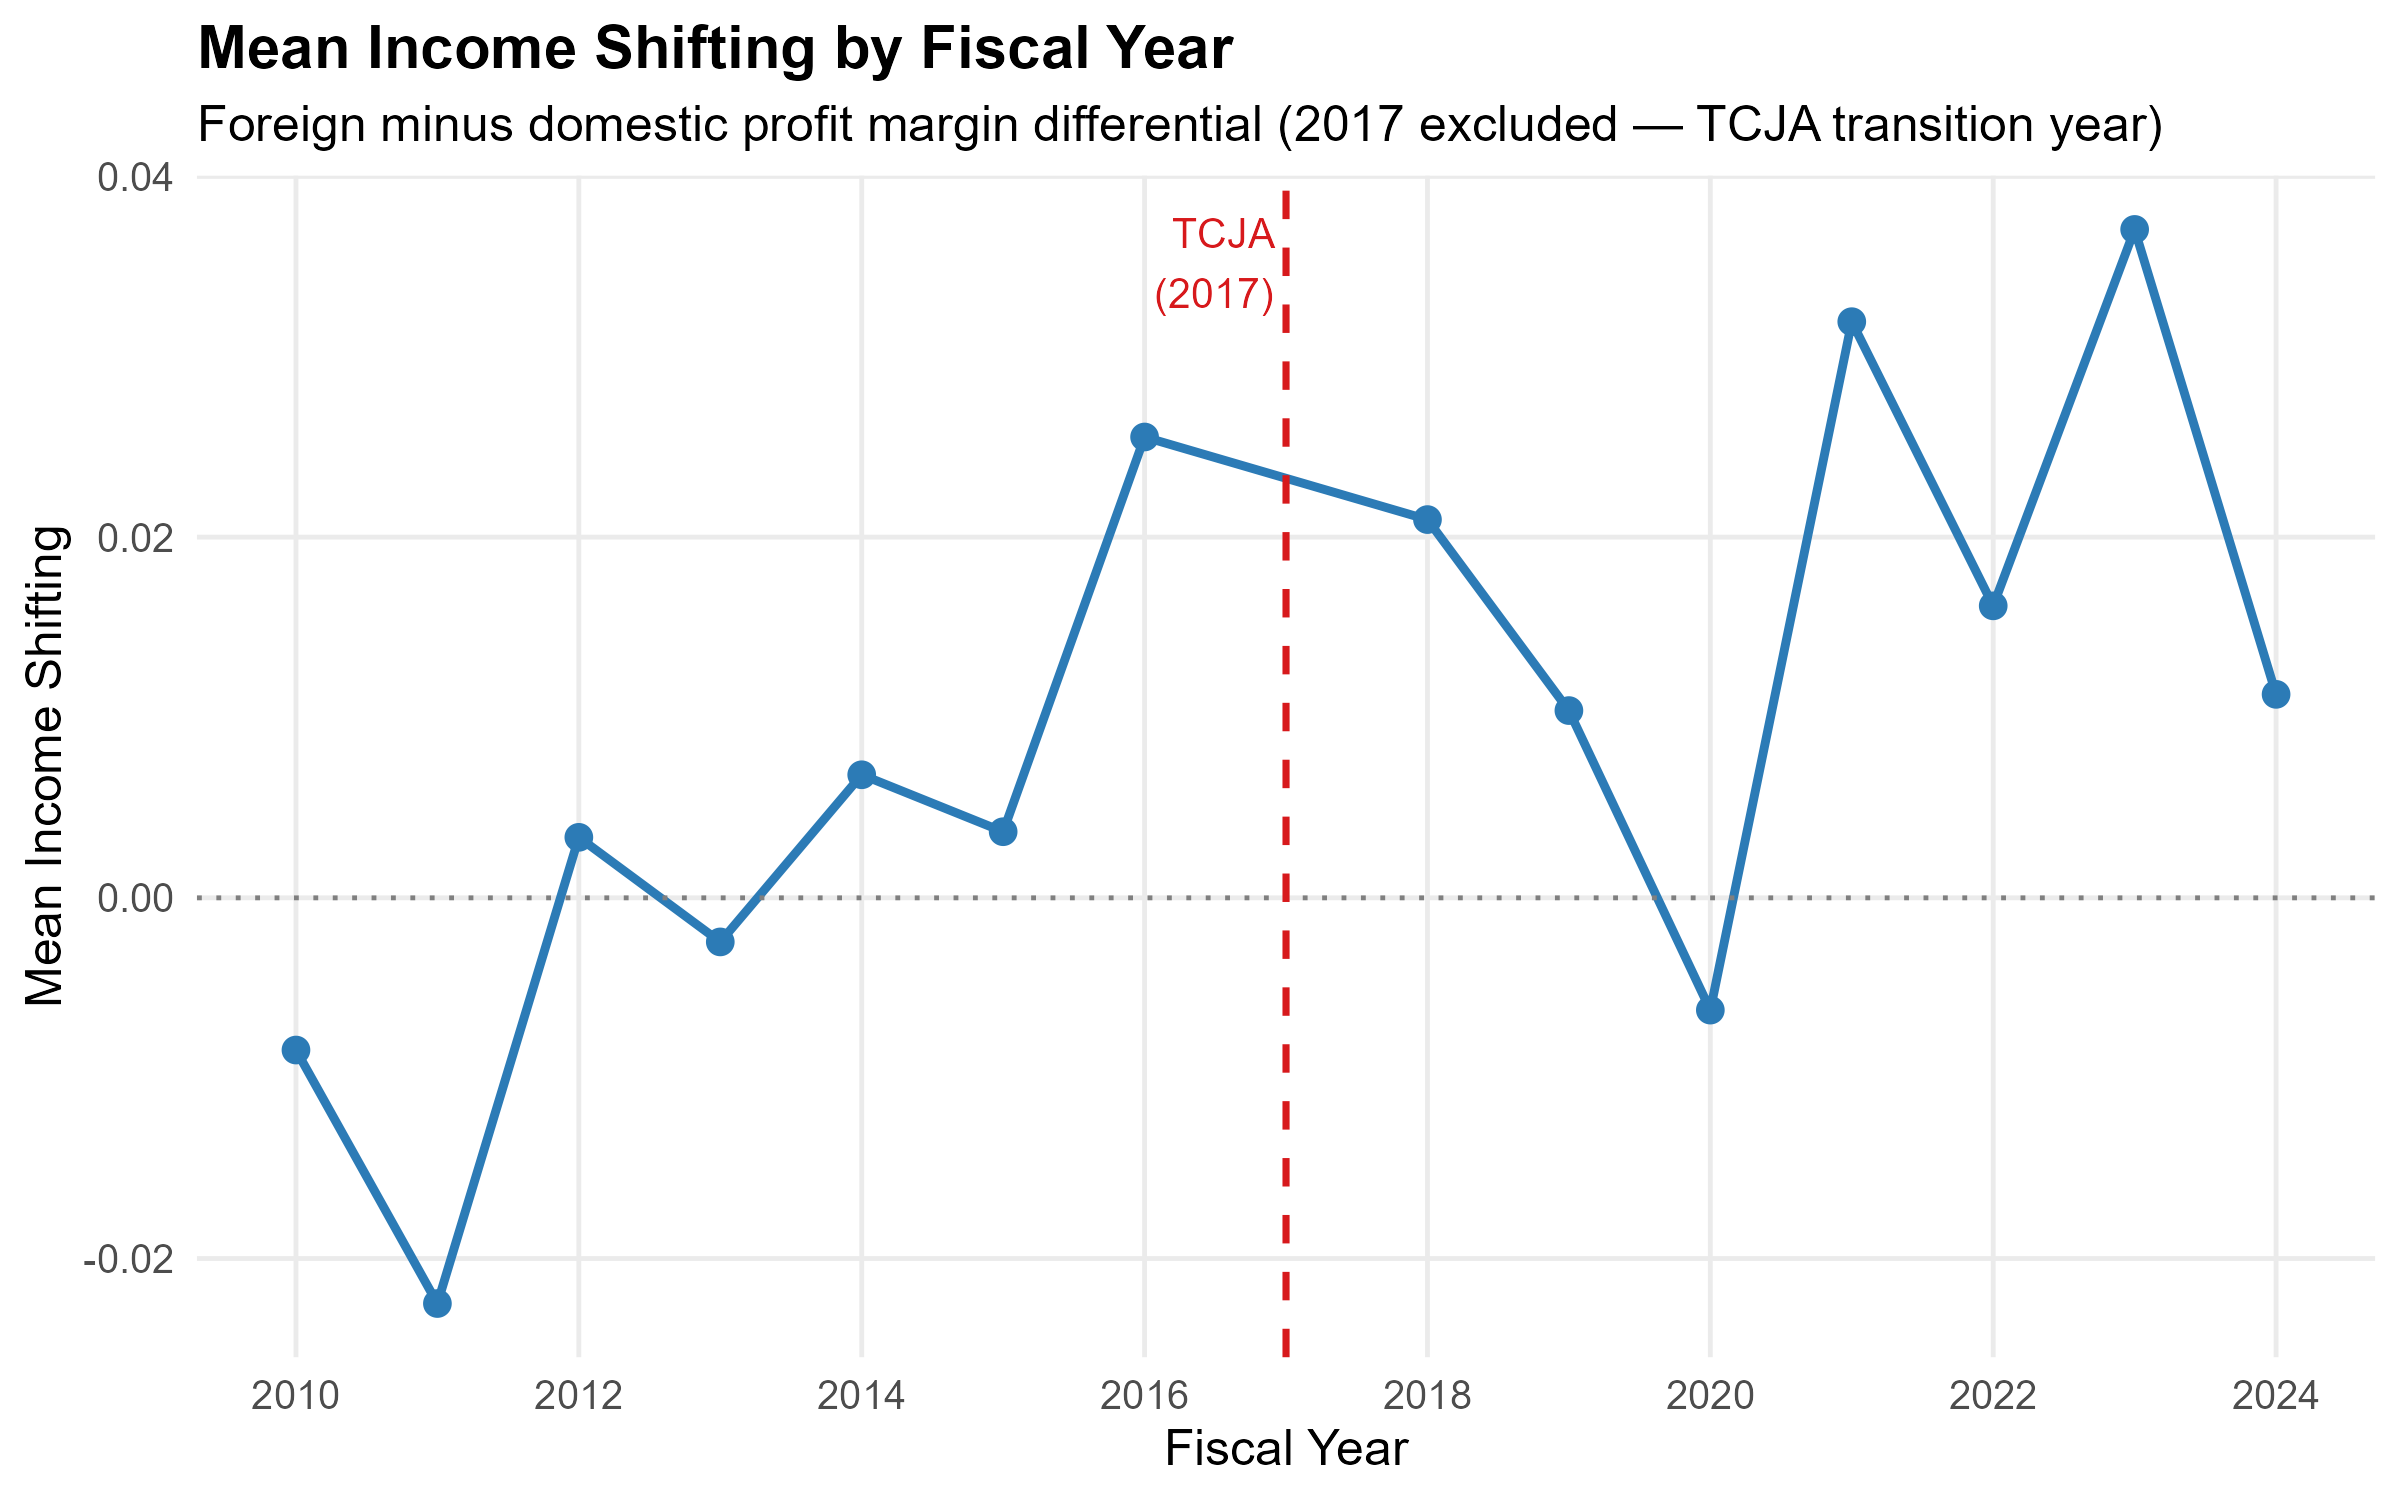
\includegraphics[width=0.9\textwidth]{fig1_income_shift_over_time.png}
\caption{Mean Income Shifting by Fiscal Year}
\label{fig:shift_time}
\end{figure}

% --- Figure 2: Tax Differential vs. Income Shifting ---
\begin{figure}[H]
\centering
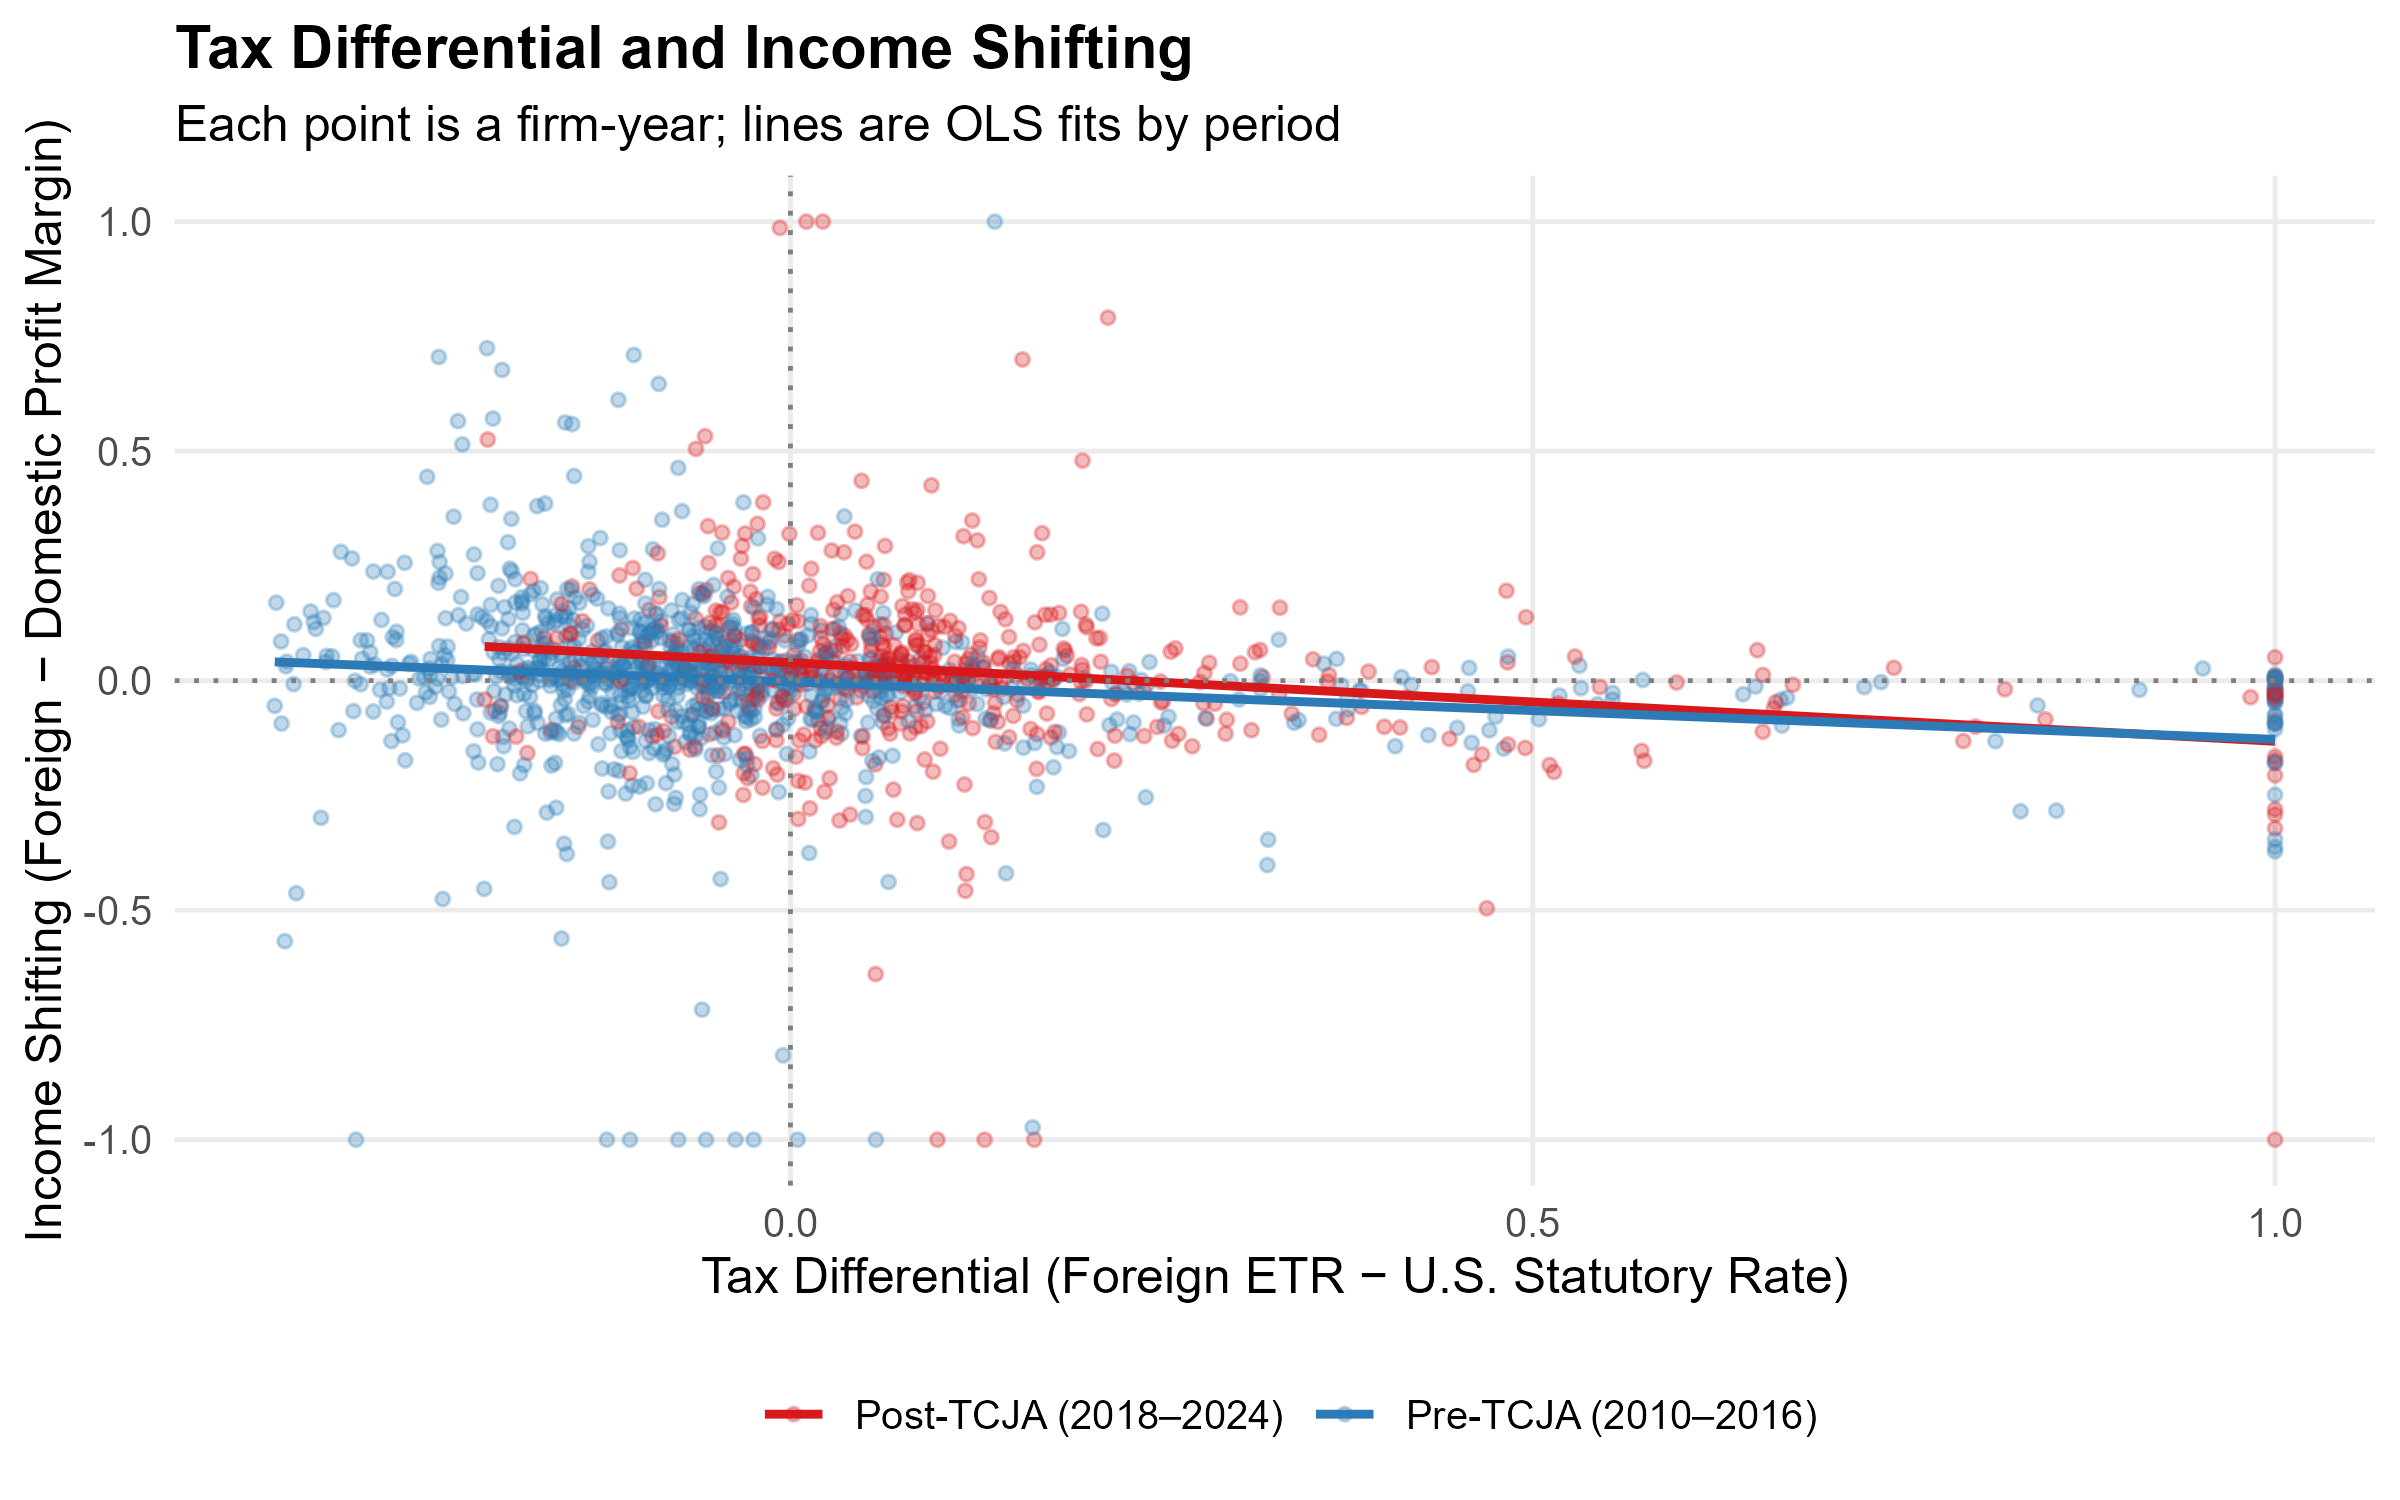
\includegraphics[width=0.9\textwidth]{fig2_tax_diff_vs_shift.png}
\caption{Tax Differential and Income Shifting by TCJA Period}
\label{fig:tax_scatter}
\end{figure}


\end{document}
